\begin{figure*}
\centering
\framebox[2.43in]{\subfloat[G]{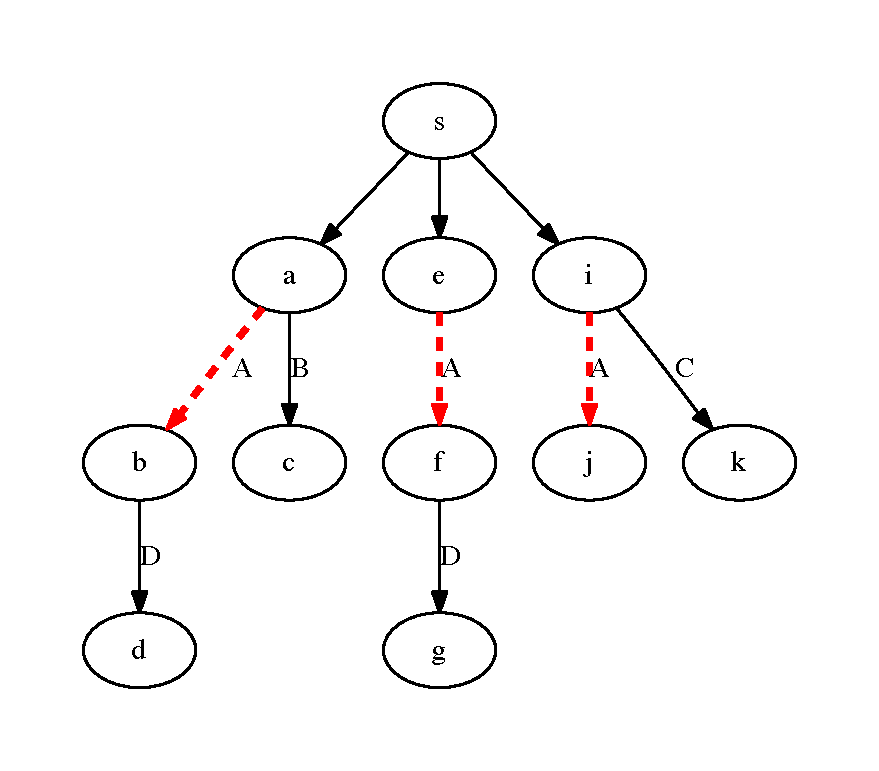
\includegraphics[width=2.4in]{nondeterminism/init.pdf}}}
\framebox[1.92in]{\subfloat[1-merge(G, a, e)]{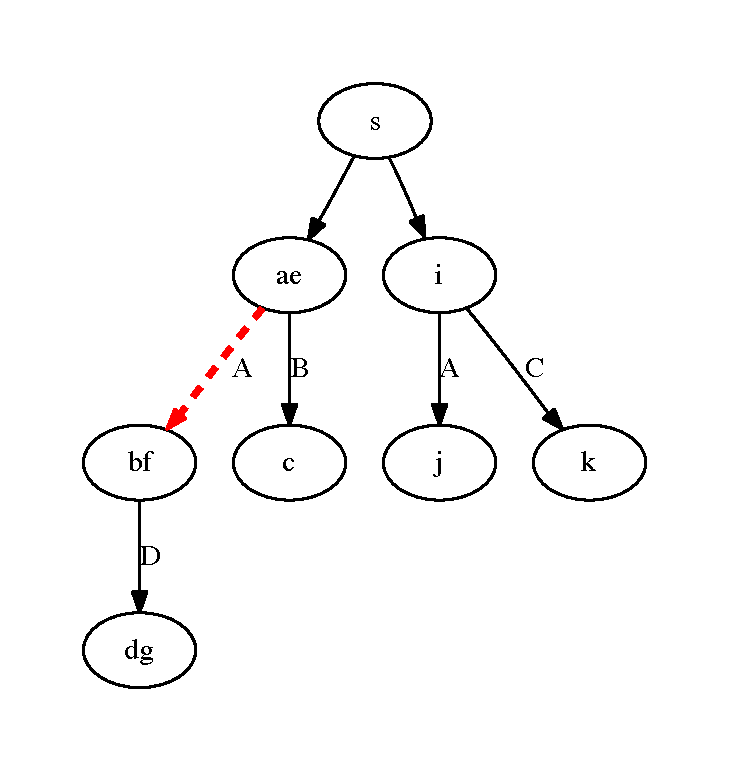
\includegraphics[width=1.9in]{nondeterminism/ae.pdf}}}
%\hspace{-.1in}
\framebox[1.92in]{\subfloat[1-merge(G, i, e)]{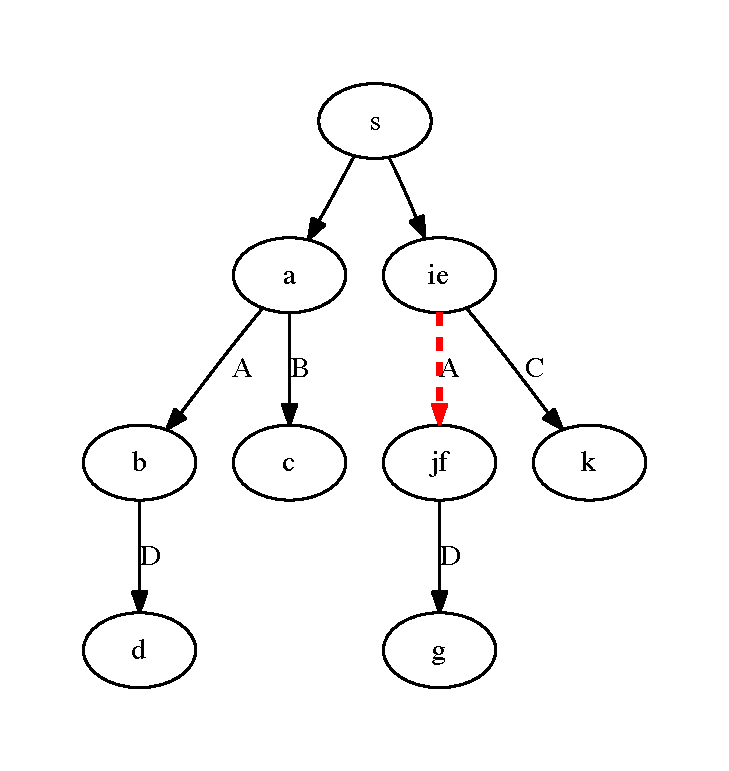
\includegraphics[width=1.9in]{nondeterminism/ie.pdf}}}
\caption{During merge, nodes may be merged in different orders, and
  order matters. That is, merging is non-associative.  Consider the
  graph in \textbf{(a)} above. The result of executing 1-equiv(G) is
  \{(a, e), (i, e)\}. That is, node pairs (a, e) and (i, e) are
  1-equiv. The dashed edges in \textbf{(a)} indicate this
  equivalence. Executing 1-merge(G, a, e) produces \textbf{(b)}
  above. In this graph node ae is not 1-equiv to node
  i. Executing 1-merge(G, i, e) produces \textbf{(c)} above. In this
  graph too, nodes a and ie are not 1-equiv. In \textbf{(b)} and
  \textbf{(c)}, bolded nodes indicate merged nodes, and the red dashed
  edge indicates the merged edges from \textbf{(a)}.}
\label{fig:gk_nondeterministic_merge}
\end{figure*}

\begin{table}[!t]
\begin{tabular}{lll}
  \textbf{Invariant} & \textbf{LTL$^-$ formula} & \textbf{Type}\\
\hline
  $x$ AlwaysFollowedBy $y$ & $\Box(x~\rightarrow~\Diamond{y})$ & liveness\\
  $y$ AlwaysPrecededBy $x$ & $\Box(y~\rightarrow~\Diamond^-{x})$ & safety\\
  $y$ NeverAfter $x$ & $\Box(x~\rightarrow~\Box{\neg{y}})$ & safety\\
\end{tabular}

\caption{Three types of detected invariants with corresponding LTL$^-$
  formula and classification. These invariants are required to be never violated
  in the course of coarsening or refinement. In LTL, $\Box$ and
  $\Diamond$ mean \emph{for all time}, and \emph{eventually}
  respectively.}

\label{table:invariants}
\end{table}


%%%%%%%%%%%%%%%%%%%%%%%%%%%%%%%%%%%%%%%%%%%%%%%%%%%%%%%%%%%%%%%%%%%%%
\section{Decision Engine}
\label{sec:decision_engine}
%%%%%%%%%%%%%%%%%%%%%%%%%%%%%%%%%%%%%%%%%%%%%%%%%%%%%%%%%%%%%%%%%%%%%

A variety of decisions that the graph refinement and coarsening
algorithms have to make are encapsulated in the decision engine. For
instance, the decision engine decides when the refinement or the
coarsening process is considered complete. These decisions are
encapsulated in the interface exposed by the decision engine to the
algorithms. We now overview the three methods comprising this
interface and the policies supported by each of these methods.

\subsection{\textit{checkGraphValidity}}

The first important decision is whether the graph is considered a
valid representation of the input traces. For this purpose the
decision engine provides the method \emph{checkGraphValidity}, defined
as

$$
checkGraphValidity~:~Graph\rightarrow{Boolean}
$$

The decision engine can use different metrics to judge whether a
representation is valid or not. Our only heuristic at the moment is to
make sure that the representation satisfies a set of temporal
invariants mined from the original input trace.

\subsubsection{Temporal Invariants Satisfaction}

The temporal relations between messages are potentially related to
their causal dependencies. Because of this we intuit that strict
temporal invariants should be preserved in the final representation of
the trace. As an example, in the two phase commit protocol, the
message TXAbort is sent \textit{because} a node sent Abort, thus
TXAbort occurs \textit{after} Abort.

\paragraph{Mining invariants.} 

We mine the patterns listed in Table~\ref{table:invariants} from the
original input traces with the temporal relation between messages
extrapolated from the timestamps. These patterns are partially based
on the specification patterns and the classification scheme formulated
by Dwyer et. al.~\cite{SpecPatterns}. Our algorithm first constructs
the temporal graph with nodes representing messages, and then
constructs the transitive closure of this graph. The invariants in
Table~\ref{table:invariants} can then be deduced by considering all
the outgoing and incoming transitions of a node. As an example,
Appendix~\ref{appendix:twopc_invariants} lists all the temporal
invariants mined for the two-phase commit protocol.

\paragraph{Checking an input graph.} The mined invariants are checked
against the input graph and True is returned only if the graph
satisfies all of them.

% On top of that, we connect messages that belong to communication
% between the same nodes.



\subsection{\textit{getMerge}}

The second method exposed by the decision engine relates to graph
coarsening. Intuitively, the purpose of this method is to break ties in the 
coarsening algorithm when there is a number of potential states to merge. 
The \emph{getMerge} method takes as input a graph and a
set of subsets of the nodes in the graph that are potential candidates
for merging (i.e. which the algorithm is capable of merging). This
method returns the element from the input set of subsets, which is the
candidate the coarsening algorithm should merge. However, this method
does not guarantee that the graph $G'$ obtained after merging will
satisfy $checkGraphValidity(G')$. Validity may not be satisfied because
this method has no information about the transformation that will be performed
on the graph by the coarsening algorithm.

$$
getMerge~:~Graph\times{\mathcal{P}(\mathcal{P}(S))}\rightarrow{\mathcal{P}(S)}
$$

This method takes a set of possible merges as argument, and returns
the best possible merge candidate set.

\subsubsection{Choose to-merge partition at random}

Our current policy to decide which nodes to merge is to pick a node at
random. For GK-Tail, this results in the behavior specified in the
original paper~\cite{AGSBM}. However, the shape of the resulting graph
depends on the random choice, and the algorithm is thus
non-deterministic. To see this, consider
Figure~\ref{fig:gk_nondeterministic_merge}. In graph \textbf{(a)},
node e is 1-equiv to nodes a and i, where 1-equiv is defined in
section~\ref{subsec:gk_tail_coarsening}. Merging nodes e and a results
in graph \textbf{(b)}, while merging e and i results in graph
\textbf{(c)}. Graphs \textbf{(b)} and \textbf{(c)} are topologically
different, and nodes ae and i in \textbf{(b)} as well as nodes ie and
a in \textbf{(a)} are not 1-equiv. Moreover graph \textbf{(b)} is a
more compact representation than graph \textbf{(c)}. The choice of
which nodes to merge, therefore, has important implications -- a
non-deterministic choices is not guaranteed to find the global
minimum, and the choice is not symmetrical. These properties can be
directly attributed to the fact that $k$-quiv is not an equivalence
relation, since it is based on subsumption, and not equivalence, of
graphs.

% The algorithm finds a local minimal representation of the traces, but
% may miss a more concise representation due to an unfortunate choice of
% the nodes to merge.

\subsection{\textit{getSplit} Policies}

The final method relates to how the graph can be refined. The
\emph{getSplit} method takes as input the graph and outputs a node and
a predicate to be applied on the node that determines the split. This
method can only be applied if there is at least some node that can be
partitioned further. getSplit is defined as

$$
getSplit~:~Graph\rightarrow{Predicate\times{}S}
$$

This method takes a graph as argument, and returns a node, and a
predicate. The predicate partitions the nodes in two sets, and this is
the intended split. There are several possibilities for deciding on
both, the node and the predicate to use for the split.

% The predicates can be grouped into two major categories: behavioral
% properties such as the presence of a certain transition, and
% structural properties, such as having a certain value in a data
% field.

% \subsubsection{Choose a node to split at random}

% We can use the node to split at random. While this is guaranteed to
% eventually lead to a graph that satisfied the invariants, it may not
% result in the smallest such graph. Since the algorithm may stop
% splitting as soon as a call to \textit{checkGraphValidity} returns
% true, the final result is non-deterministic in this case, too.

\subsubsection{Counter-example guided}

An informed method to select the state to split is to use
counter-example to the invariants that were initially mined. For every
unsatisfied invariant, there is a violating trace, and the node to
split can be chosen from such a trace. There are several possible ways
to choose the node. In Bikon we pick the first violating node from the
trace. We do so because it provides us with an intuitive measure of
progress -- splitting the first violating node leads us to hope that
the resulting paths have no violations, or have at least one fewer
violating nodes. The predicate returned by getSplit is the transition
in the invalid path.

%  to use for splitting can be either a behavioral
% property, such as the presence of a certain transition in the node, or
% a structural property, such as certain values in data fields.



